%\subsection{Basic Net Architecture}
%We wanted to evaluate the quality of basic features. For some features we tried multiple different architectures to compare them among themselves. 
To evaluate the quality of our features, we've implemented different architectures to compare them with each other.
%That resulted in seven \textit{basic models} (BM). Each of the models has an ID for referencing within the further text.
%All models have single or related features as input and generate a binary classification output using sigmoid as our activation function.
All seven models use single or related features as input and generate a binary classification output using sigmoid as the activation function. Each of the models has an ID which will be used as reference within the further text.

\subsection{Architectures}

\paragraph{Model 1} This model takes the article headline as input. We normalized the headline length and embedded the words using an embedding layer which we initialized with pretrained glove embeddings \cite{pennington2014glove}. The model uses a dense and batch normalization layer as hidden layer.
\paragraph{Model 2} Like BM 1 this model takes the article headline as input. Instead of a dense layer this one uses a convolutional layer with kernel sizes one, tree and five as well as a pooling layer as proposed by Y. Kim \cite{kim2014convolutional}.
\paragraph{Model 3} This model takes the first words of the article text. They get embedded the same way as in BM 1 and BM 2 and processed through an LSTM layer outputting the last cell state.
\paragraph{Model 4} This model takes the article category as input. The category id gets embedded using an embedding layer and processed through a dense and a batch normalization layer.
\paragraph{Model 5} This model takes temporal features of the publication as input. The features are minute, hour, day of the week and day of the year. The features get processed the same way as in BM 4.
\paragraph{Model 6} This model takes the headline and the article word count. From both of them the logarithm is calculated. The logarithm is used to create exponential sized bins for different lengths. Each logarithm gets embedded and processed like in BM 5 and 6.
\paragraph{Model 7} This model takes the competitive score \ref{eq:competitive_score} and processes it through a dense layer as well as batch normalization.

\subsection{Training}
We split the dataset into training, validation and test sets using a 70/15/15 split with respect to the timestamps of publication. We chose this split because in a real world scenario the whole set would be used to train the model and predictions would happen on future articles.

Because our task implies a strongly imbalanced training set we used class weights. They influence the weighting of the loss while training indirectly proportional to the class size of a giving training sample.

\subsection{Combined Net Architecture}
We combined the BMs to use multiple features and improve our results. The decision on what models are combine worthy we calculated the correlations between each BM pair using the predictions for the test data set, shown in Figure \ref{fig:correlation_matrix}. Furthermore we included the performance of each model in our consideration. Taking the correlations and the performance into account we decided on a larger set of combined models.The combined models share their classification layers but not the hidden layers.

\begin{figure}
	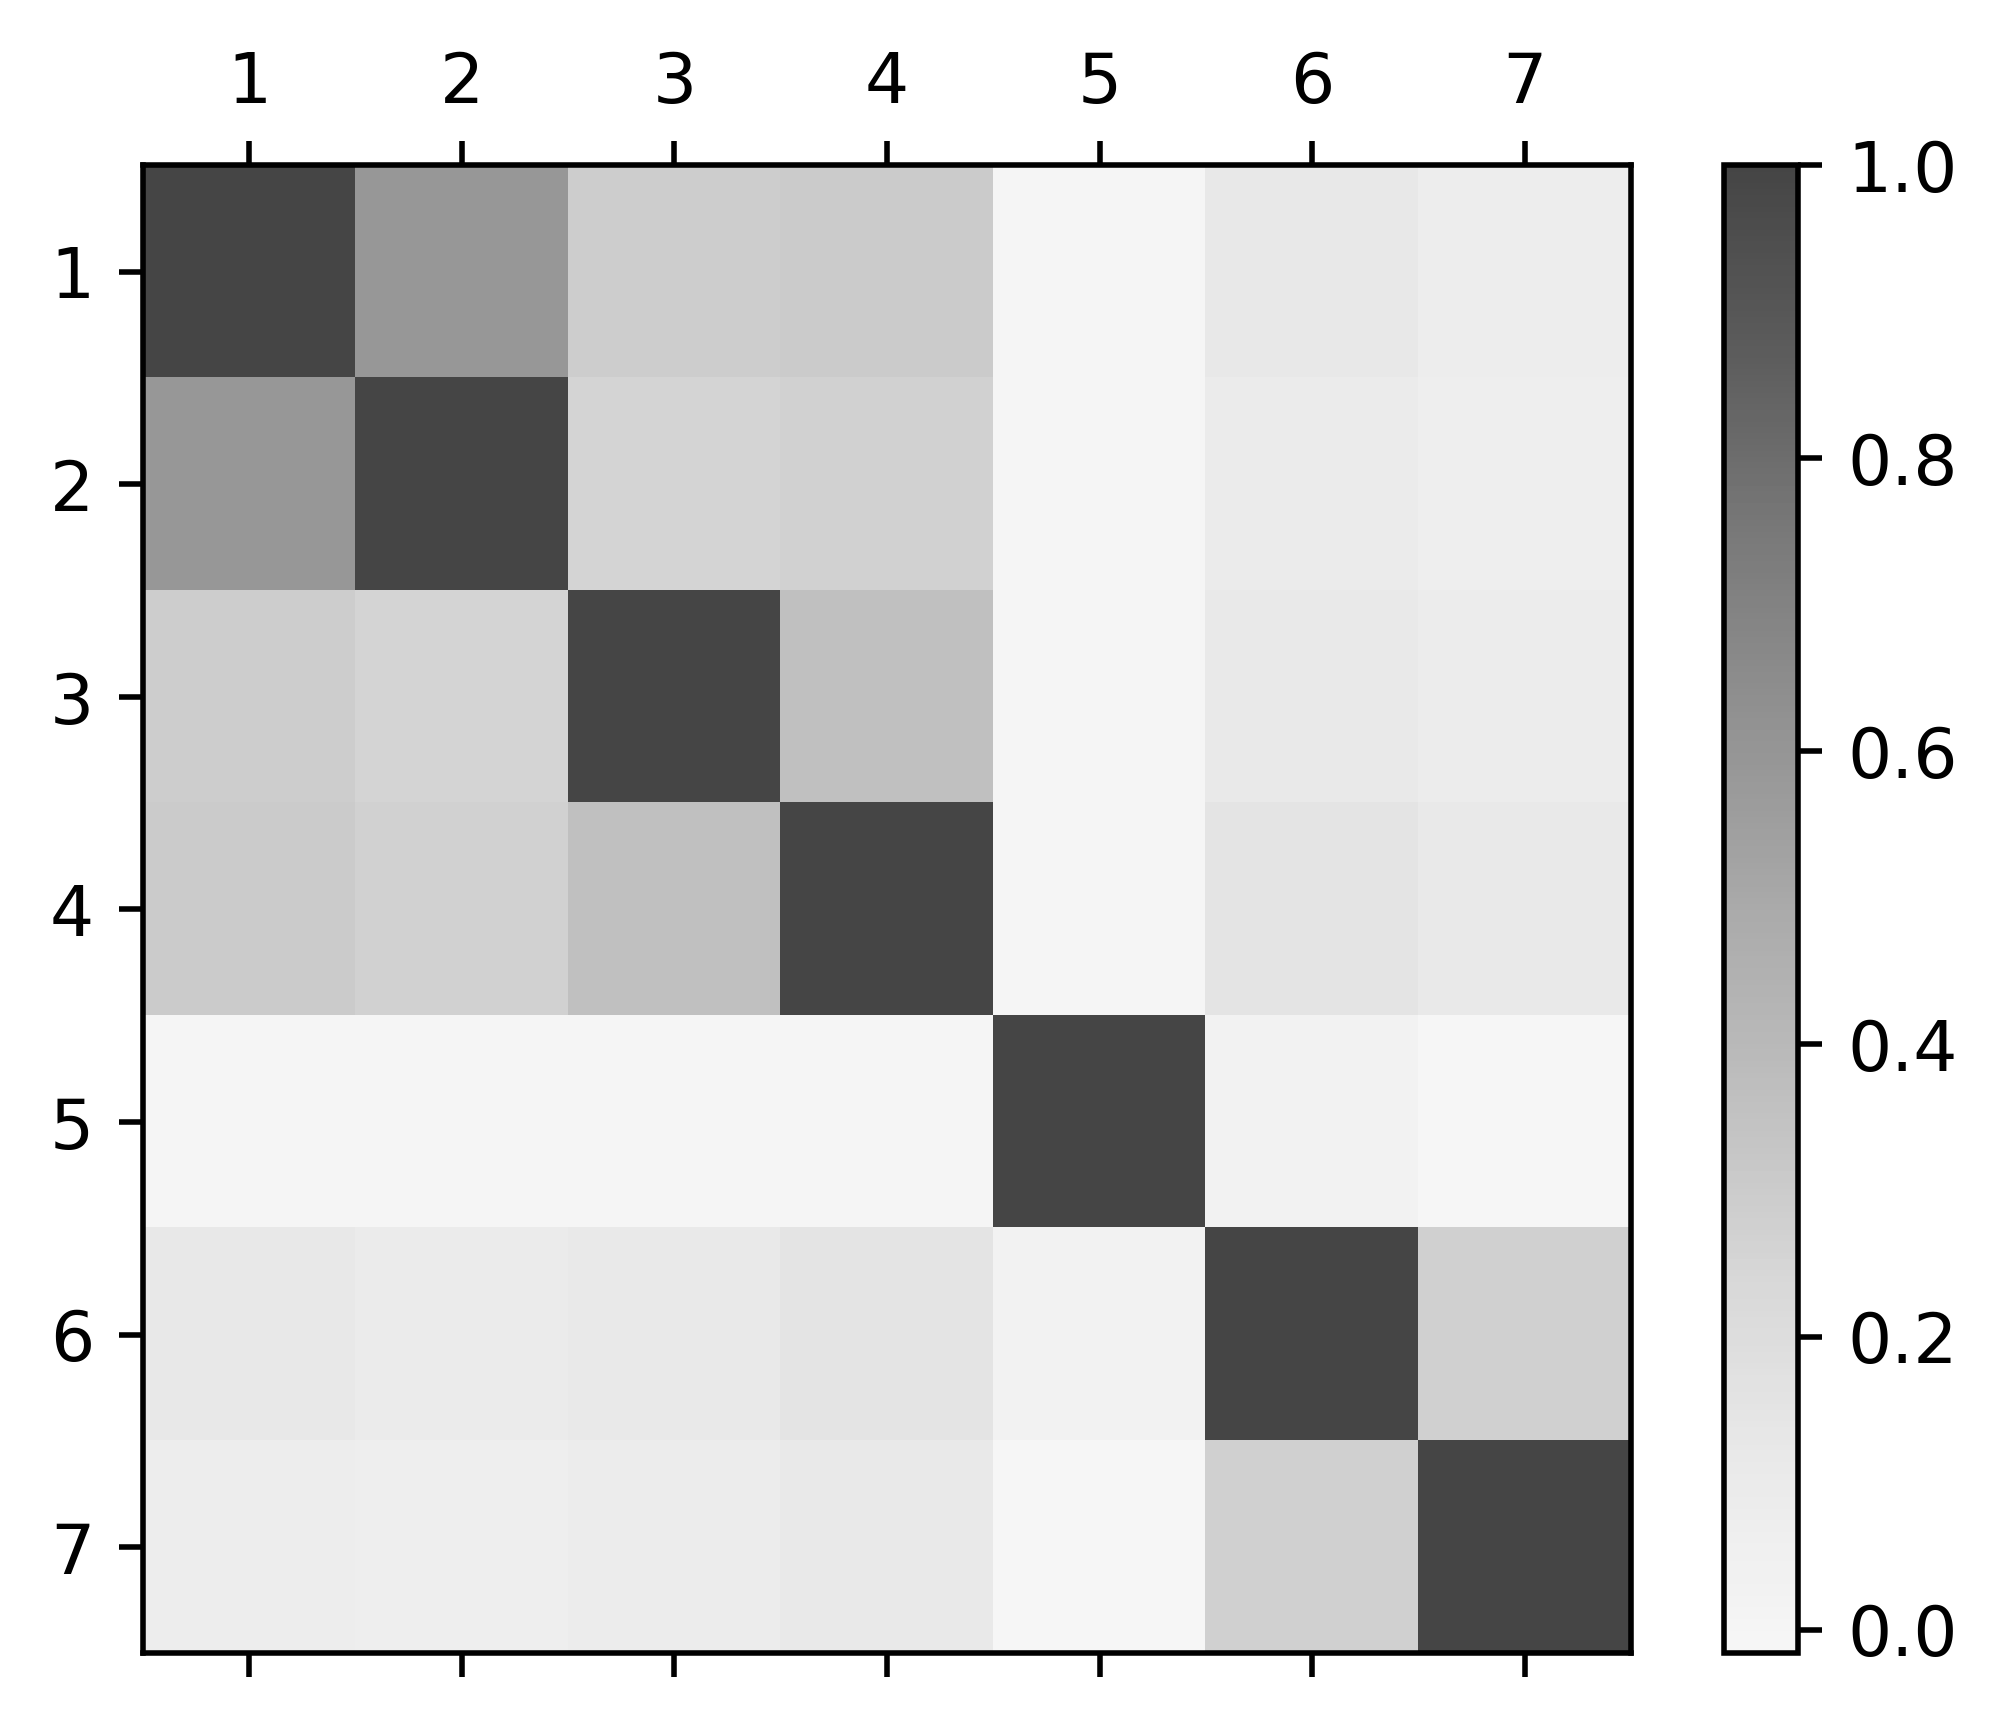
\includegraphics[width=0.5\textwidth]{fig/correlations_bw.png}
	\caption{Correlation matrix of the basic models.}
	\label{fig:correlation_matrix}
\end{figure}